\documentclass[a4paper,12pt]{article}

% Input Encoding
\usepackage[utf8]{inputenc}
% Margin Controls
\usepackage[a4paper,bottom=3cm,left=2cm,right=2cm,top=2cm]{geometry}
% Hyphenation libraries
\usepackage[british]{babel}
\usepackage{hardwrap}

% Layout and graphics libraries
\usepackage{graphicx}
\usepackage{wrapfig}
\usepackage{multicol}
\usepackage{tabularx}
\usepackage{url}
\usepackage[perpage,symbol*,bottom,hang,multiple]{footmisc}
\usepackage{tikz}
\usepackage{pdflscape}
\usepackage{etoolbox}
\usepackage{lipsum}
\usetikzlibrary{patterns}

% Page style
\pagestyle{plain}
\newcommand{\fixparskip}{\setlength{\parskip}{4mm plus1mm minus1mm}}
\fixparskip
\setlength{\parindent}{0pt}
\setlength{\columnsep}{1cm}
\renewcommand{\arraystretch}{2}

% Article Environment
\newcommand{\articleAuthor}{}
\newenvironment{article}[2]{
	\pagebreak[2]
	\renewcommand{\articleAuthor}{#2}
	
	{\Huge#1}

	}{

	\notblank{\articleAuthor}{\hfill\Large\articleAuthor}{}
	\vspace{12mm}
	}

\begin{document}
% Title Page
\begin{center}
~ % Non-breaking space so that the page starts, and \vfill evaluates
\vfill

\includegraphics[width=\textwidth,height=0.7\textheight,keepaspectratio]{pictures/cover}
\vfill

\resizebox{!}{16mm}{Picocon 34}

\resizebox{!}{10mm}{Futurism}\\
\vspace{1mm}
%\resizebox{!}{6mm}{\it{ }} %Use to add subtitle e.g. 'In Medias Res' (Picocon 33)

\vspace{5mm}
\resizebox{!}{8mm}{Wyrmtongue}

\thispagestyle{empty}
\end{center}
\clearpage
% End of title page


\begin{article}{The King's Speech}{Henry Wild - ICSF Chair}
	Greetings all, and welcome to the 35th Annual Picocon!

My team of minions have organised a fantastic event for you all, with talks by some awesome guests, some smashing of the dodgiest merch around (although anyone seen harming adorable little porgs will have to face my wrath), and a chance to appreciate some of the worst works of the genre for charity. There's also definitely not a fish duel, and we're actually definitely not erecting a statue in Anurag's honour. 

It has been a great year for the society so far, with many fun and new events, such as the introduction of Themed Fridays and a recent collab with AstroSoc. We encountered a few technical difficulties with converting the library into Atlantis (books + water = bad), which provoked a super sing-a-long ICSF Tour round the various Union Meeting Rooms. We even have T-Shirts to prove it! Apologies if the library isn't in its usual pristine condition - debates over the most efficient sorting algorithm for reshelving the books have yet to be solved. We have plenty of fun events planned for the rest of the term, which are detailed somewhere in this Wyrm. I hope to see you there!

So now it just remains for me to wish you a merry Picocon and a happy smashing things dipped in liquid nitrogen!
\end{article}

\begin{article}{The Sofa's Ramblings}{Elizabeth Windo - Picocon Sofa}
	Dearest attendees, I am your sofa for today.
A sofa, whilst more comfortable than a chair, is not as applicable to every situation. While the chair handles the everyday business, the sofa is brought out to receive honoured visitors. These would be you, dearest attendees.
Welcome to the floor show.

Today has been a work in progress for slightly more than three hundred and sixty five days, with the first strands being drawn together at Picocon 33 a year ago. Whilst last year, we looked behind towards our origins, this year we look towards our future – or the future of those that may come after.  This is both narratively attractive, and relevant. Private space exploration is a very real possibility in the next few years,  with drone landings governed by a CEO that acknowledges the necessity for intrasolar colonisation in the short term. Computers seem to be better at moving small monochrome rocks in specific patterns than people are.  Numbers as large as 21 can now be factorised in polynomial time. The layperson may wonder, what next? Where will we go from here? We may not know yet, but it’s going to be interesting finding out.

We have a plethora of writers for your enjoyment whose works have touched upon topics from unconstrained artificial intelligence to environmentally friendly space colonisation.

Our first speaker, Jaine Fenn, has an extensive history both with science fiction and technology. Her talk will cover the future of science fiction as a medium – and explain ‘Why Sci-Fi Rules the Page’.  Al Robertson’s subsequent talk, `Into heaven, out of hell’, will cover his two books, discussing the inspirations and observations made within them and seeing how the predictions made seem to be turning out given the events between now and the time of writing.  After this, Paul McAuley will discuss his past and current work, and offer some insight into how the saucer books of the 1960s shaped his view on extraterrestrial entities in his talk `Aliens: a short personal history’.  Finally, we have Justina Robson. Her talk, ``Artificial Intelligence: if you want to scare yourself silly, get a future'' is about her journey thinking through both AI and philosophical ramifications - and how that feeds into her books.

Organising this event has been Fun, a word that here means `chaotic and all-consuming’. However, it would not have been possible without my right and left hands, the beanbag and the chair of vice. They have been instrumental in assembling the day that is ahead. I also wish to thank the many volunteers, committee members, and administrative whizzes who have put their time and sanity into this event. Every person in this list has been invaluable, and I am immensely grateful to all of them.

A warm welcome to you all. Live long and prosper.

\end{article}

\begin{article}{A Word from the Beanbag}{Edward Da Fonesca - Picocon Beanbag}
	Twisted is a celebration of the subversive nature of tales spun by storytellers, through the loom of words, screen and anything in between. It’s been a whirlwind to organise, but I enjoyed every convoluted minute of it and hope you do too. Between the GoH’s twisty talks and a variety of loopy games and activities, you’re sure to be entertained.

During the day, you might find yourself meandering on the curling complexities of life, from nautili to black holes. But be careful \textendash{} if you spiral too hard, you might become aware of something more, coiling around the reality you know and waiting patiently with twisted intent for you to slip up. I’m afraid it may already be too late.
\end{article}

\pagebreak
\begin{article}{What's On}{}
	For those of you who don't know, there are many fun events to attend at Picocon. As well as talks by all the Guests of Honour, there is an Author’s Panel where the authors can be asked questions by the attendees. Silly Games is an event where we imitate various gameshows, with general hilarity ensuing, and the Tabletop and Gaming societies run activities as well. We also have an event known simply as ‘Harmless Fun’. 

There are charity events in collaboration with RAG, such as Turkey Readings and Viewings, where books or films are read/shown, but they are so bad that people will pay to prevent them from continuing (or to make it keep going!). We also have ‘Destruction of Dodgy Merchandise’ (DoDM), where examples of terribly misguided merchandise are bid on to be saved or dunked in liquid notrogen and smashed by the highest bidder – the proceeds again going to charity. This year, as last year, Stuart Ashens is coming to Imperial from the Youtube domain to chair the auctioning of the merchandise.

In the evening there will be a showing of the film Le Voyage Dans La Lune, which was the first science-fiction film on the screen, and a Pub Quiz, with the teams captained by our illustrious Guests of Honour! 

We have booksellers and various retailers of items from jewellery to professionally illustrated prints by Autun Purser, and our own stand selling Picocon 33 t-shirts with this year’s logo.
\end{article}

\begin{article}{Futurism}{ }
	 Futurism has been defined in many ways – for a while it was an artistic movement aiming to liberate Italy from the mistakes of the past. For a while, it was a relentlessly optimistic dream about a society free from resource constraints, becoming in some places a more cynical view based on extrapolating current societal trends to their presumed conclusion. At heart however, it has always been about us, and about what these trends mean for humanity.

In 2010, the price of the textbook `The making of a fly’ was \$70. For a brief time in 2011, it was \$2.4 million. Rather than this being an art piece with the intent of making some scathing indictment of overpriced textbooks, it was entirely the result of a rather stupid pricing system. Two antagonistic market algorithms escalated and escalated until a stable position was reached – or rather, until the owners noticed the absurdity and shut it down. This is an absurd example, but it highlights the problems with poorly specifying the implementation of an algorithm – a harmless situation in this toy case, but one which has far reaching implications.

The day has come where the existence of machine learning \& artificial intelligence affects more than a single edge case, and instead affects large parts of society. It already affects us.  It affects the institutions and communities we live within, and with advances in medicine, it may in future affect the fundamental qualities of our bodies. If we as a society survive to that point, then it will be rather interesting to see what happens.

A still more glorious dawn awaits?
\end{article}

\begin{article}{Predicting Picocon}{ }
	All good speculative convention fiction requires predictions about how things will be in the future. Usually, this is done by learned experts,  such as past sofas, or people on the street. However, science has given us the power to change this. With the powers of modern computer science, we can predict what future Picocons will look like by extrapolating from past ones. Using a naive Bayes model, where the choice of which letter to use is given by the probability that we’ve seen that letter before, we can predict who the guests of honour will be and even the theme of the convention.

The most statistically likely list of predicted guests of honour follows:
\begin{enumerate}
\item	AL
\item	AL
\item	AL
\end{enumerate}

Apparently Al is a common name for guests of honour, to the extent that our system predicts that the entire world will be consumed by an organisation of Al based life forms.

The best guess for the theme of the convention will be WALFIBBFET.
We’re not quite sure what this means at all.

It is clear that technology is still some way from accurately predicting Picocon. However, as machine learning progresses (and future years give us more data to train the algorithm with). Until them, we may simply have to wait and see.

\end{article}

\pagebreak

\begin{article}{Tabletop Gaming at Picocon!}{B\'{a}lint Babik - Chair, Imperial College Tabletop Gaming Society}
	This year the Tabletop Gaming society will be running boardgames and RPGs in Meeting Room 3 of the union (enter the main entrance, take the lift up to the 3rd floor and the door is on your right). Boardgames will run from 14:30 (just after the author’s panel) until late, where we have lots and lots of games available, short and long to match everyone’s tastes.  We have some of our members around to teach games too, so don’t worry if you don’t know any from our collection.
 
We will also have some role playing games running in meeting room 3 from 18:00! No experience required, just bring your imagination. These will start promptly so please arrive at 6pm or as soon as possible afterwards.
 
Tabletop has regular Boardgame, RPG and Magic events each week of term. Check out our facebook group to find out where and when: www.facebook.com/groups/ImperialCollegeBoardGames/


\end{article}
\begin{article}{Gaming}{Ariana Sadr-Hashemi – Chair, Imperial College Gaming Club}
	Imperial College Gaming Club may not be associated with the Science Fiction society in any official sense, but we’ve shared a reasonable number of members within the past few years and I myself have many a reason to appreciate Sci-Fi, so the natural step from there is to run something at Picocon.

We’ll have our games consoles set up in Meeting Rooms 1 and 2 from 16:00 – 17:00, and again once all other events have ended at 19:00. We’ll be running our most popular games – namely Super Smash Bros. and Just Dance (it’s much more fun than it sounds). Whether you’re a regular member of Gaming, wanting to reignite an old passion, or even if you haven’t touched a video game in years, I can guarantee you’ll have fun. There’s a good reason why video games are one of the leading causes of procrastination in the country.

And if you happen to be a student, and you’re not yet aware of us (read: if I haven’t pestered you to come to Gaming before), you may like to know that the Club meets on a regular basis, on Wednesdays from 2pm in Room 403A in the EEE building.

I hope you all enjoy Picocon, and find discover/confirm your passion for video games when you come and see us.


\end{article}

\clearpage
\begin{article}{Schedule}{}
	\vspace{2mm} {\Large} \nopagebreak
\raggedright
\begin{center}
\begin{tabularx}{13cm}{c X l}

09:00 & Front Desk/Registration Opens\footnotemark[1] & \\
09:30 & Author's Talk - Paul Cornell\footnotemark[2] & \\
%10:00& \\
10:30 & Author's Talk - Carrie Hope Fletcher\footnotemark[2]\\
%11:00 & \\
11:30 & Author's Talk - Michelle Paver\footnotemark[2]\\
%12:00 & \\
12:15 & Destruction of Dodgy Merchandise \footnotemark[1]&\\
12:30 & Lunch (see Menu)\footnotemark[3] &\\
%13:00 & \\
13:30 & Author's Panel\footnotemark[2] & \\ 
%14:00 & \\
14:30 & Turkey Readings and Silly Games\footnotemark[2], Boardgames begin \footnotemark[4]&\\
%15:00 & \\
%15:30 & \\
16:00 & Gaming \footnotemark[5]\\
%16:30 & \\
17:00 &  Harmless Fun \it(definitely not a fish duel)\footnotemark[1] &\\
17:30 & Film Showing: \it{Le Voyage Dans La Lune}\footnotemark[3] &\\
18:00 & Pub Quiz (with authors leading teams!) \footnotemark[3], RPGs begin \footnotemark[4]& \\
\end{tabularx}
\end{center}

\footnotetext[1]{Beit Quad}
\footnotetext[2]{Blackett LT1}
\footnotetext[3]{568 and Metric}
\footnotetext[4]{Tabletop gaming events in Meeting Room 3. These will run until late.}
\footnotetext[5]{Meeting Rooms 1 and 2}

\end{article}

\vspace{- 2 cm}

\begin{article}{Lunch details}{}
	Food will be served between 12:30-13:30 in Metric, from a mobile servery. Food tickets can be purchased in FiveSixEight and redeemed at the Metric servery. Prices below:

Beef Burger and Chips -£4.75\\
Chicken Burger and Chips - £4.80\\
Veggie Burger and Chips - £4.25\\
Mediterranean roasted vegetable and tomato pasta - £3.95\\
Please note, anyone purchasing any other items from the menu will need to wait as normal as these will be prepared in the main kitchen.
\end{article}

\clearpage

\begin{article}{Guests of Honour}{}
{\Large Jaine Fenn}

\begin{wrapfigure}{r}{4cm}
	\vspace{-10mm}
	\resizebox{4cm}{!}{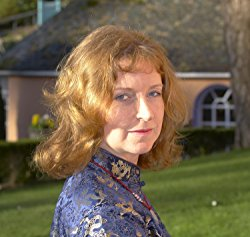
\includegraphics{pictures/fenn}}
	\vspace{-10mm}
\end{wrapfigure}

Jaine Fenn is the author of numerous published short stories and the Hidden Empire series of character-driven Space Opera novels. After studying linguistics and astronomy her first career was in IT, an experience which has left her with a distrust of technology unusual in an SF author. She was originally a guest at Picocon in 2009, shortly after the first Hidden Empire book, Principles of Angels, came out from Gollancz. Her talk, 'Why SF Rules the Page' will discuss the relevance of science-fiction, and how it continues to be a relevant and insightful medium.
\\ \\
{\Large Paul McAuley}

\begin{wrapfigure}{r}{4cm}
	\vspace{-10mm}
	\resizebox{4cm}{!}{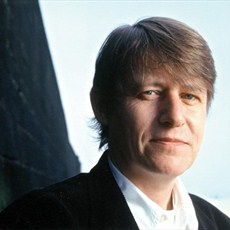
\includegraphics{pictures/paul-mcauley}}
	\vspace{-10mm}
\end{wrapfigure}

Paul McAuley, one of the most widely-praised authors in British science fiction, has published more than twenty novels, over a hundred short stories, and a BFI Film Classic monograph on Terry Gilliam’s film Brazil. His fiction has been nominated for numerous prizes and has won the Arthur C. Clarke Award, the Philip K Dick Memorial Award, and many others. After working as a research biologist and university lecturer in botany, he is now a full-time writer.
\\ \\
{\Large Al Robertson}

\begin{wrapfigure}{r}{4cm}
	\vspace{-10mm}
	\resizebox{4cm}{!}{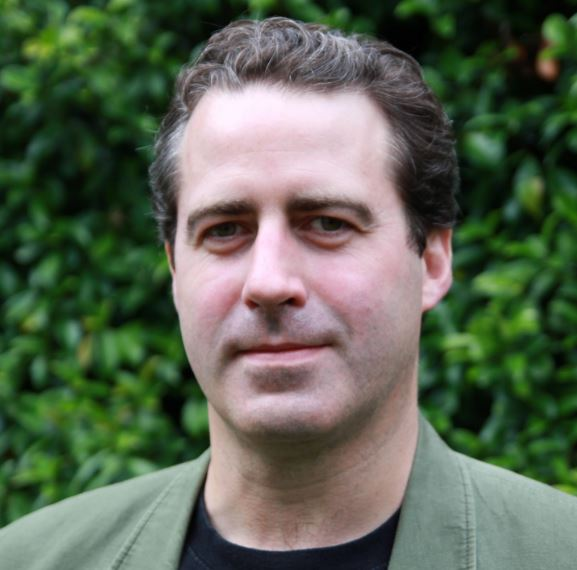
\includegraphics{pictures/al-robertson}}
	\vspace{-10mm}
\end{wrapfigure}

Al Robertson is a writer, poet, and marketer, whose first novel, `Crashing Heaven', came out last June. His second novel, `Waking Hell’, was released last October with Gollancz. He's been publishing SF, fantasy and horror stories and novellas for the last ten years or so - these have appeared in Interzone, Black Static, Postscripts and elsewhere.  His talk, `Into Heaven, Out of Hell’, will cover his two books, discussing the inspirations and observations made within them and seeing how the predictions made turned out.  
\\ \\
{\Large Justina Robson}

\begin{wrapfigure}{r}{4cm}
	\vspace{-10mm}
	\resizebox{4cm}{!}{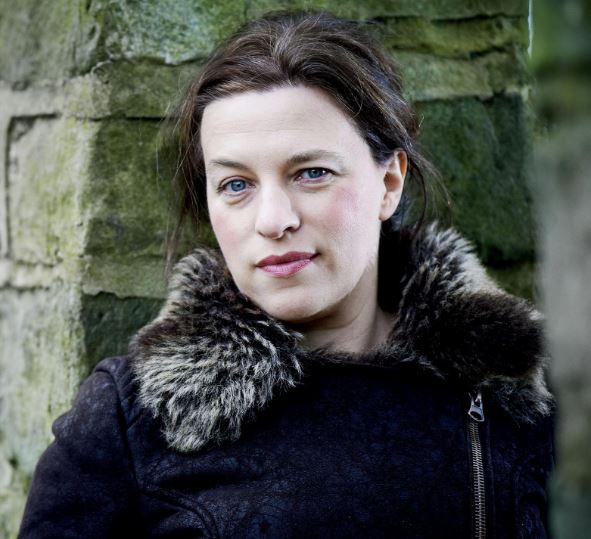
\includegraphics{pictures/justina-robson}}
	\vspace{-10mm}
\end{wrapfigure}

Justina Robson has spent a lot of her life writing Science Fiction. This has included ten novels, a collection of short stories, and a Transformers book. Her debut novel, Silver Screen, was shortlisted for the Arthur C Clarke award and the BSFA award. She currently lives in Leeds. Her talk, "Artificial Intelligence: if you want to scare yourself silly, get a future." is about her journey thinking through both AI and and philosophical ramifications - and how that feeds into her books.
\clearpage
{\Large Stuart Ashen}

\begin{wrapfigure}{r}{4cm}
	\vspace{-10mm}
	\resizebox{4cm}{!}{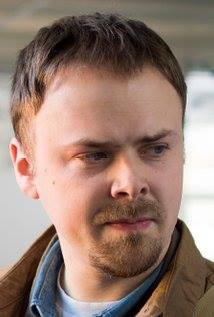
\includegraphics{pictures/ashens}}
	\vspace{-10mm}
\end{wrapfigure}

Stuart Ashen, or Ashens, is an enigma. He has single handedly compiled over 50 thousand shades of the colour gray. He has produced over 520 videos. Today, he will harness the power of liquid nitrogen to destroy an assortment of terrifyingly ill designed merchandise. Truly, anything is possible for Stuart Ashen. We are honoured, if slightly scared, to welcome him again today.
%	\begin{tabular}{p{\dimexpr\columnwidth}}
%	\\
%		{\Large Jaine Fenn}

\begin{wrapfigure}{r}{4cm}
	\vspace{-10mm}
	\resizebox{4cm}{!}{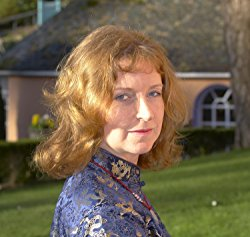
\includegraphics{pictures/fenn}}
	\vspace{-10mm}
\end{wrapfigure}

Jaine Fenn is the author of numerous published short stories and the Hidden Empire series of character-driven Space Opera novels. After studying linguistics and astronomy her first career was in IT, an experience which has left her with a distrust of technology unusual in an SF author. She was originally a guest at Picocon in 2009, shortly after the first Hidden Empire book, Principles of Angels, came out from Gollancz. Her talk, 'Why SF Rules the Page' will discuss the relevance of science-fiction, and how it continues to be a relevant and insightful medium.
%
%		\vspace{4cm} ~
%	\\
%		{\Large Paul McAuley}

\begin{wrapfigure}{r}{4cm}
	\vspace{-10mm}
	\resizebox{4cm}{!}{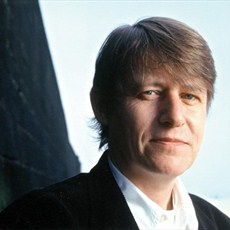
\includegraphics{pictures/paul-mcauley}}
	\vspace{-10mm}
\end{wrapfigure}

Paul McAuley, one of the most widely-praised authors in British science fiction, has published more than twenty novels, over a hundred short stories, and a BFI Film Classic monograph on Terry Gilliam’s film Brazil. His fiction has been nominated for numerous prizes and has won the Arthur C. Clarke Award, the Philip K Dick Memorial Award, and many others. After working as a research biologist and university lecturer in botany, he is now a full-time writer.
%
%		\vspace{4cm} ~
%	\\
%		{\Large Al Robertson}

\begin{wrapfigure}{r}{4cm}
	\vspace{-10mm}
	\resizebox{4cm}{!}{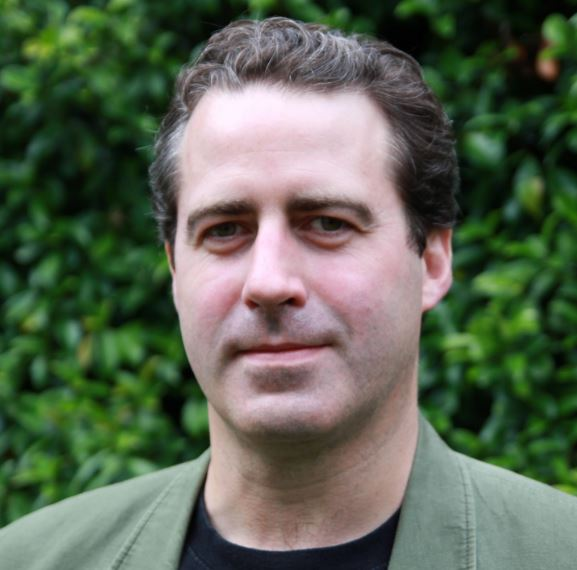
\includegraphics{pictures/al-robertson}}
	\vspace{-10mm}
\end{wrapfigure}

Al Robertson is a writer, poet, and marketer, whose first novel, `Crashing Heaven', came out last June. His second novel, `Waking Hell’, was released last October with Gollancz. He's been publishing SF, fantasy and horror stories and novellas for the last ten years or so - these have appeared in Interzone, Black Static, Postscripts and elsewhere.  His talk, `Into Heaven, Out of Hell’, will cover his two books, discussing the inspirations and observations made within them and seeing how the predictions made turned out.  
%
%		\vspace{4cm} ~
%	\\
%		{\Large Justina Robson}

\begin{wrapfigure}{r}{4cm}
	\vspace{-10mm}
	\resizebox{4cm}{!}{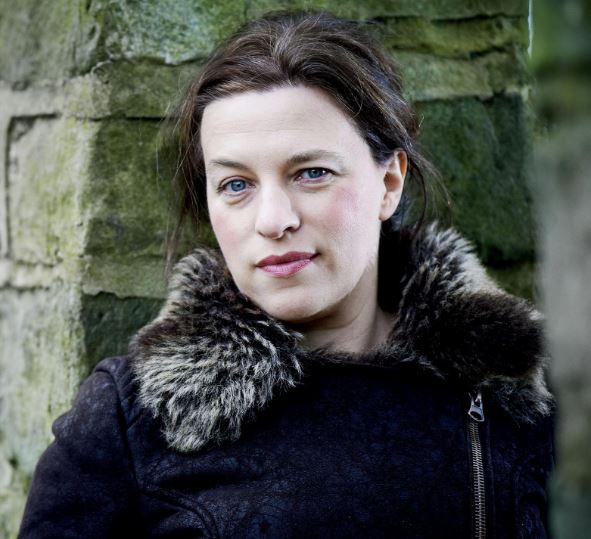
\includegraphics{pictures/justina-robson}}
	\vspace{-10mm}
\end{wrapfigure}

Justina Robson has spent a lot of her life writing Science Fiction. This has included ten novels, a collection of short stories, and a Transformers book. Her debut novel, Silver Screen, was shortlisted for the Arthur C Clarke award and the BSFA award. She currently lives in Leeds. Her talk, "Artificial Intelligence: if you want to scare yourself silly, get a future." is about her journey thinking through both AI and and philosophical ramifications - and how that feeds into her books.
%
%		\vspace{4cm} ~
%	\\
%		{\Large Stuart Ashen}

\begin{wrapfigure}{r}{4cm}
	\vspace{-10mm}
	\resizebox{4cm}{!}{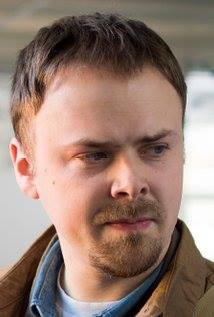
\includegraphics{pictures/ashens}}
	\vspace{-10mm}
\end{wrapfigure}

Stuart Ashen, or Ashens, is an enigma. He has single handedly compiled over 50 thousand shades of the colour gray. He has produced over 520 videos. Today, he will harness the power of liquid nitrogen to destroy an assortment of terrifyingly ill designed merchandise. Truly, anything is possible for Stuart Ashen. We are honoured, if slightly scared, to welcome him again today.
%	\end{tabular}
\end{article}

\clearpage

\begin{article}{Vendors}{}
	Our vendors are located on the second floor of the Blackett foyer, and and would love to introduce themselves to you.

\vspace{5mm}

{\Large Paul Couper}

A reader/collector of SF/Fantasy, selling at Picocon to clear duplicates built up whilst collecting and upgrading. My collection is now over 12,000 paperbacks, but still has many gaps. Most wanted at present? Probably E Pluribus Unicorn, Theodore Sturgeon, Timescape paperback (i.e. 4th Pocket printing) to complete my timescape collection. So if anyone has a copy of that (or other collectables) for sale, wants to buy, or indeed just wants a chat, stop by during the day.

\vspace{5mm}

{\Large Clockwork Firebird Designs - Alex Locke }

Welcome to Clockwork Firebird Designs! I am a self-taught, ever-evolving tailor, leather worker and costume maker with a penchant for creating monsters. I attend Live Action Role-Play (LARP) events and Anime/Comic conventions as both a trader and attendee on a regular basis. I've been doing leather work since 2008, and selling since 2011. I recall learning to sew when I was 6 years old and I've not really stopped since. Within the shop you may find armour, masks, trinkets, painted artworks, soft toys... anything I bring to mind or feel like turning my hand to! I am still finding my feet, and I am always learning new techniques.

\vspace{5mm}

{\Large Blackwell Books }

This year, giving you an even greater selection of books to browse from, we will also be welcoming Blackwell's for the first time. For Picocon, they will primarily be stocking books by our Guests of Honour, so it will be a great chance for you to grab a copy of the books you've heard all about today!
\end{article}

\clearpage
\begin{article}{Quest Objectives}{}
	On your way in, you should have been assigned to one of three teams - the Omnics, the Collective, or the Jesters - and given a sticky badge to wear with newfound pride.
If somehow you slipped through the net,
or misplaced your badge,
then go and \emph{politely} berate the receptionists until they give you one.

You will find a list of dangerous, potentially impossible items below.
Find any of these items, bring the evidence back to the front desk, and win fabulous prizes... in the form of points for your team.
Whichever team ends up with the most points will be declared the finest, the greatest, and most importantly the winners!

Now go \emph{for great justice}.

This year's teams are:

\begin{tabular}{ccc}
	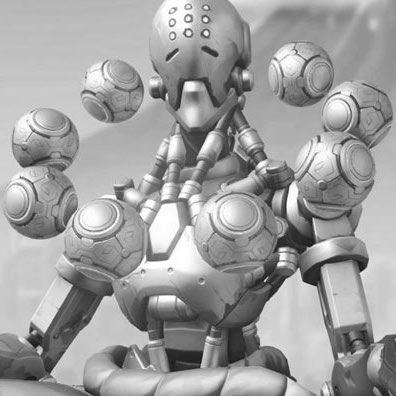
\includegraphics[width=0.2\columnwidth]{pictures/zenyatta} &
	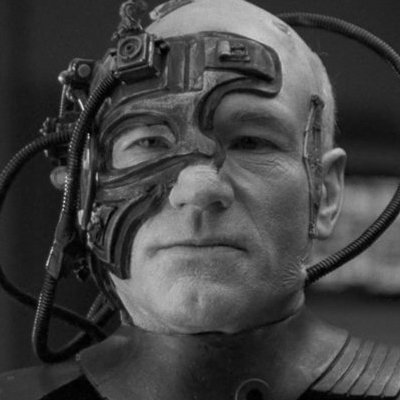
\includegraphics[width=0.2\columnwidth]{pictures/borg} &
	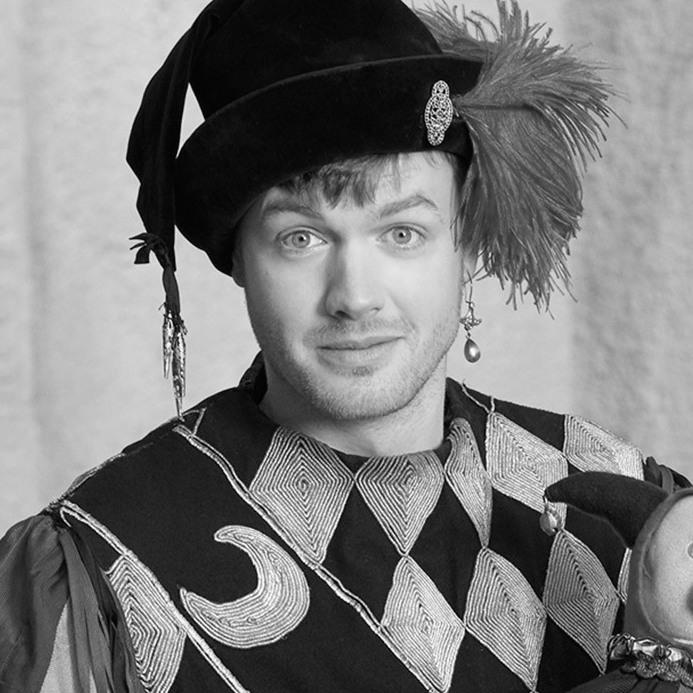
\includegraphics[width=0.2\columnwidth]{pictures/jester} \\

	\parbox{0.3\textwidth}{\center\large The Omnics - be one with the universe} &
	\parbox{0.3\textwidth}{\center\large The Collective - items will be assimilated} &
	\parbox{0.3\textwidth}{\center\large The Jesters - a hunt, but with jazz hands!} \\
\end{tabular}
\vspace{5mm}

These items can be submitted to the Front Desk for Fun Points (after 11am).
Pictures are not (generally) admissible; objective involving people {\textit
must only be undertaken with the other person's permission}.
The front desk reserves the right to keep the submitted items. Each faction may
claim an item on the only once, unless otherwise noted.
\begin{tabbing}
	FD \quad \= Front Desk Person's Discretion\footnotemark \\
	E \> This item may be claimed multiple times per faction (``each'') \\
	M \> For each faction, the highest of their scores will be used
\end{tabbing}
\footnotetext{This actually
	applies to everything; where it is noted, it indicates that you’re
	unlikely to change anyone's mind with your cunning arguments.}

\begin{multicols}{2}
	\begin{tabbing}
1 \hspace{12mm}	\= Little Green Pygmy Solders (E) \\
1	\> Hugs (per person) \\
30	\> Picocon \\
20	\> A non-ICSF fresher at Picocon \\
Age +5	\> Ex-ICSF Chair (M) \\
Age +5	\> Ex-ICSF Librarian (M) \\
Age +5	\> T-shirts from Picocons past (M) \\
10 	\> Previous Guest of Honour (E) \\
10	\> Half of one (1) Dave \\
5	\> The blood of a Picocon first-timer \\
20	\> The Mabbott set \\
8	\> A phylactery \\
80 	\> Dave Clements' phylactery \\
100	\> The Picocon Sofa, calm \\
50	\> The Picocon Beanbag, frantic \\
15	\> Tea, earl grey, hot \\
25 	\> A good drink (FD, E) \\
10 	\> A less good drink (FD) \\
-5	\> Unsatisfactory drink (FD) \\
5	\> Delicious blood (FD) \\
15	\> Spirits from beyond \\
1000 	\> £100 (E) \\
7	\> The contents of my pocketses \\
5	\> Good news (FD, E) \\
-5	\> Bad news (FD, E) \\
1	\> A funny joke (FD, E) \\
-1	\> A bad pun (FD, E) \\
10	\> A charge of EIE/EEE students \\
25	\> A competent barbershop \\ \> quartet (FD) \\
5	\> Any song sung in the style of \\ \> William Shatner \\
50	\> A barbershop quartet in the style \\ \> of William Shatner \\
50 \> Any door to London Below \\
3   \> Newly acquired merchandise  \\
5   \> A teleological proof of the\\ \> existence of a higher power \\
1   \> The solution to the next item \\ \> on the list (E) \\
-1  \> The solution to the previous \\ \> item on the list (E)\\
10  \> Donations of a themed plastic \\ \> abomination \\
5   \> A demon bear (bonus points if fluffy) \\
5   \> A member of the Family of Blood \\
5   \> A little fall of rain \\
5	\> Origami \\
20  \> Dinosaur origami \\
8	\> A Non-Euclidean triangle \\
5   \> A snake eating its own snake tail, \\ \> or snail.\\
5	\> Tribble \\
60	\> Tribble (functional) \\
5	\> A nanosecond \\
10  \> An accretion disk \\
30  \> A terrifying technological terror \\
3	\> A good hat \\
5	\> A correctly fitted top hat \\
5   \> Convincing closet cosplay \\
10  \> Convincing actual cosplay \\
10  \> Pretty trinkets (FD) \\
3   \> The start of something beautiful \\
30   \> The phone from a castle \\
20  \> The phone from a police box \\
50	\> Happiness, $\ge$ 0.1M concentration \\
n(n-1)	\> n Interlocking cogs (functional \\ \> after being poked) (M) \\
10   \> Out of place kerning \\
20   \> An unaired TV pilot \\
20   \> An untelevised air pilot \\
30 	\> A control crystal (with \\ \> demonstration) \\
40 	\> Three quarters of a planck length \\
20 	\> A demonstration of Xeno's paradox \\
10  \> An aesthetically pleasing key (FD)\\
14 	\> A clowder of one cat \\
5   \> The man they call Jayne (or his hat) \\
-50 \> The source of the mysterious ticking noise \\
400	\> The World Turtle \\
800 \> With orbiting bodies \\
10  \> A surviving member of the Imperial \\ \> Steampunk Society \\
50	\> A book ICSF lacks (and wants) \\
1	\> The light at the end of the tunnel \\
5	\> A crowning moment of awesome \\
17	\> Proof humanity's reach extends \\ \> beyond its imagination \\
70  \> A lost Doctor Who episode \\
3	\> Famous last words (subject to \\ \> checking) \\
-1	\> Anything irrelevent (E) \\
-5  \> Anything irrelephant (E) \\
4	\> An Ed (picked up) \\
3	\> Galaxy \\
2	\> A practical application for \\ \> General Relativity \\
4	\> Transcendent understanding \\
10	\> A point in the complex plane \\
5   \> A working AI (demonstrated) \\
10  \> A working AI (safely demonstrated) \\
1000	\> Time machine (points were awarded \\ \> 16th Feb 6pm, ICSF Library, \\ \> password is ``arpeggio'') \\
25	\> A swordfish \\
35	\> A fishsword \\
10	\> A Swan \\
4	\> Nerf Guns \\
3	\> NERV guns \\
10	\> Lab stuff \\
-50	\> per fatality \\
10	\> The Staff of Ra \\
3	\> Positronic brain \\
3	\> Observable Brownian Motion \\
5	\> A fluffy dragon \\
7	\> A plasma generator \\
5	\> Ion cannon (demonstrated) \\
-20	\> Spontaneous combustion \\ \> whilst dancing (E)\\
5	\> A Henry (E)\\
10	\> A Wild Henry\\
10	\> A completed nonogram\\
15	\> A completed crossword\\
	\end{tabbing}
\end{multicols}

{\large Good Luck!}

You're likely to need it...

\end{article}

\begin{article}{Nonogram}{}
	\begin{center}
POSSIBLE NONOGRAM HERE
	%	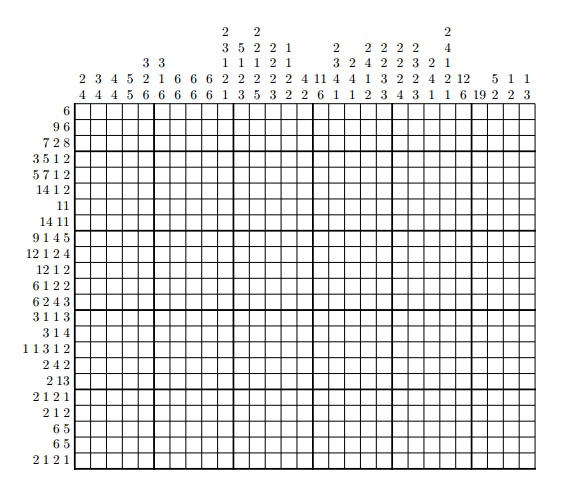
\includegraphics[width=\textwidth,height=0.5\textheight,keepaspectratio]{puzzles/nonogram.jpg}
	\end{center}
\end{article}

\pagebreak

\begin{article}{Crossword}

\begin{center}
POSSIBLE CROSSWORD HERE
%	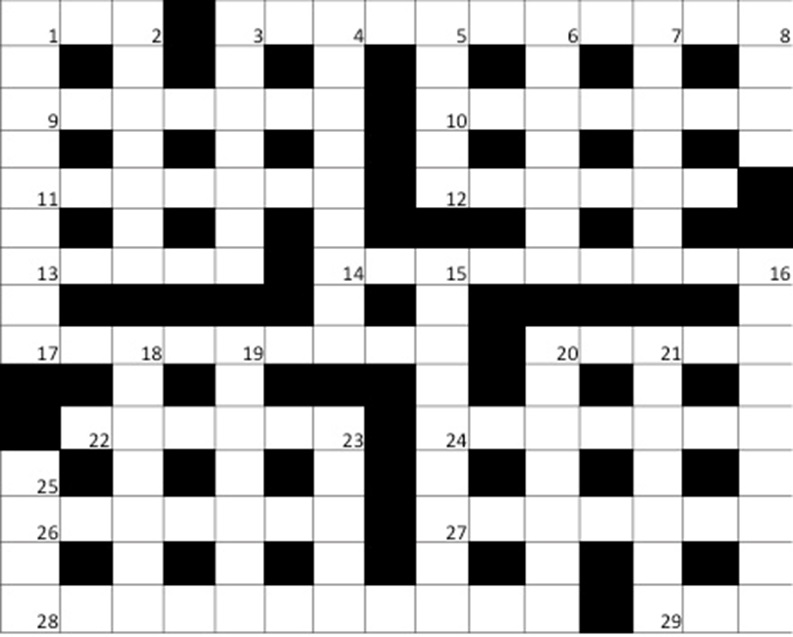
\includegraphics[width=\textwidth,height=0.5\textheight,keepaspectratio]{puzzles/crossword.jpg}
\end{center}

\begin{multicols}{2}
POSSIBLE CROSSWORD HERE
	%\input{puzzles/cword.latex}
\end{multicols}

\end{article}

\begin{article}{Map}{}
	\begin{center}
		\resizebox{\columnwidth}{!}{%  Coordinates are shifted and scaled Long/Lat values
%  (0, 0) maps to (-0.1781, 51.5)
%  Rotated clockwise, and slanted into look perpendicular
%  Values have been pre-multipled by 100 to make sure there's no undeflow issues

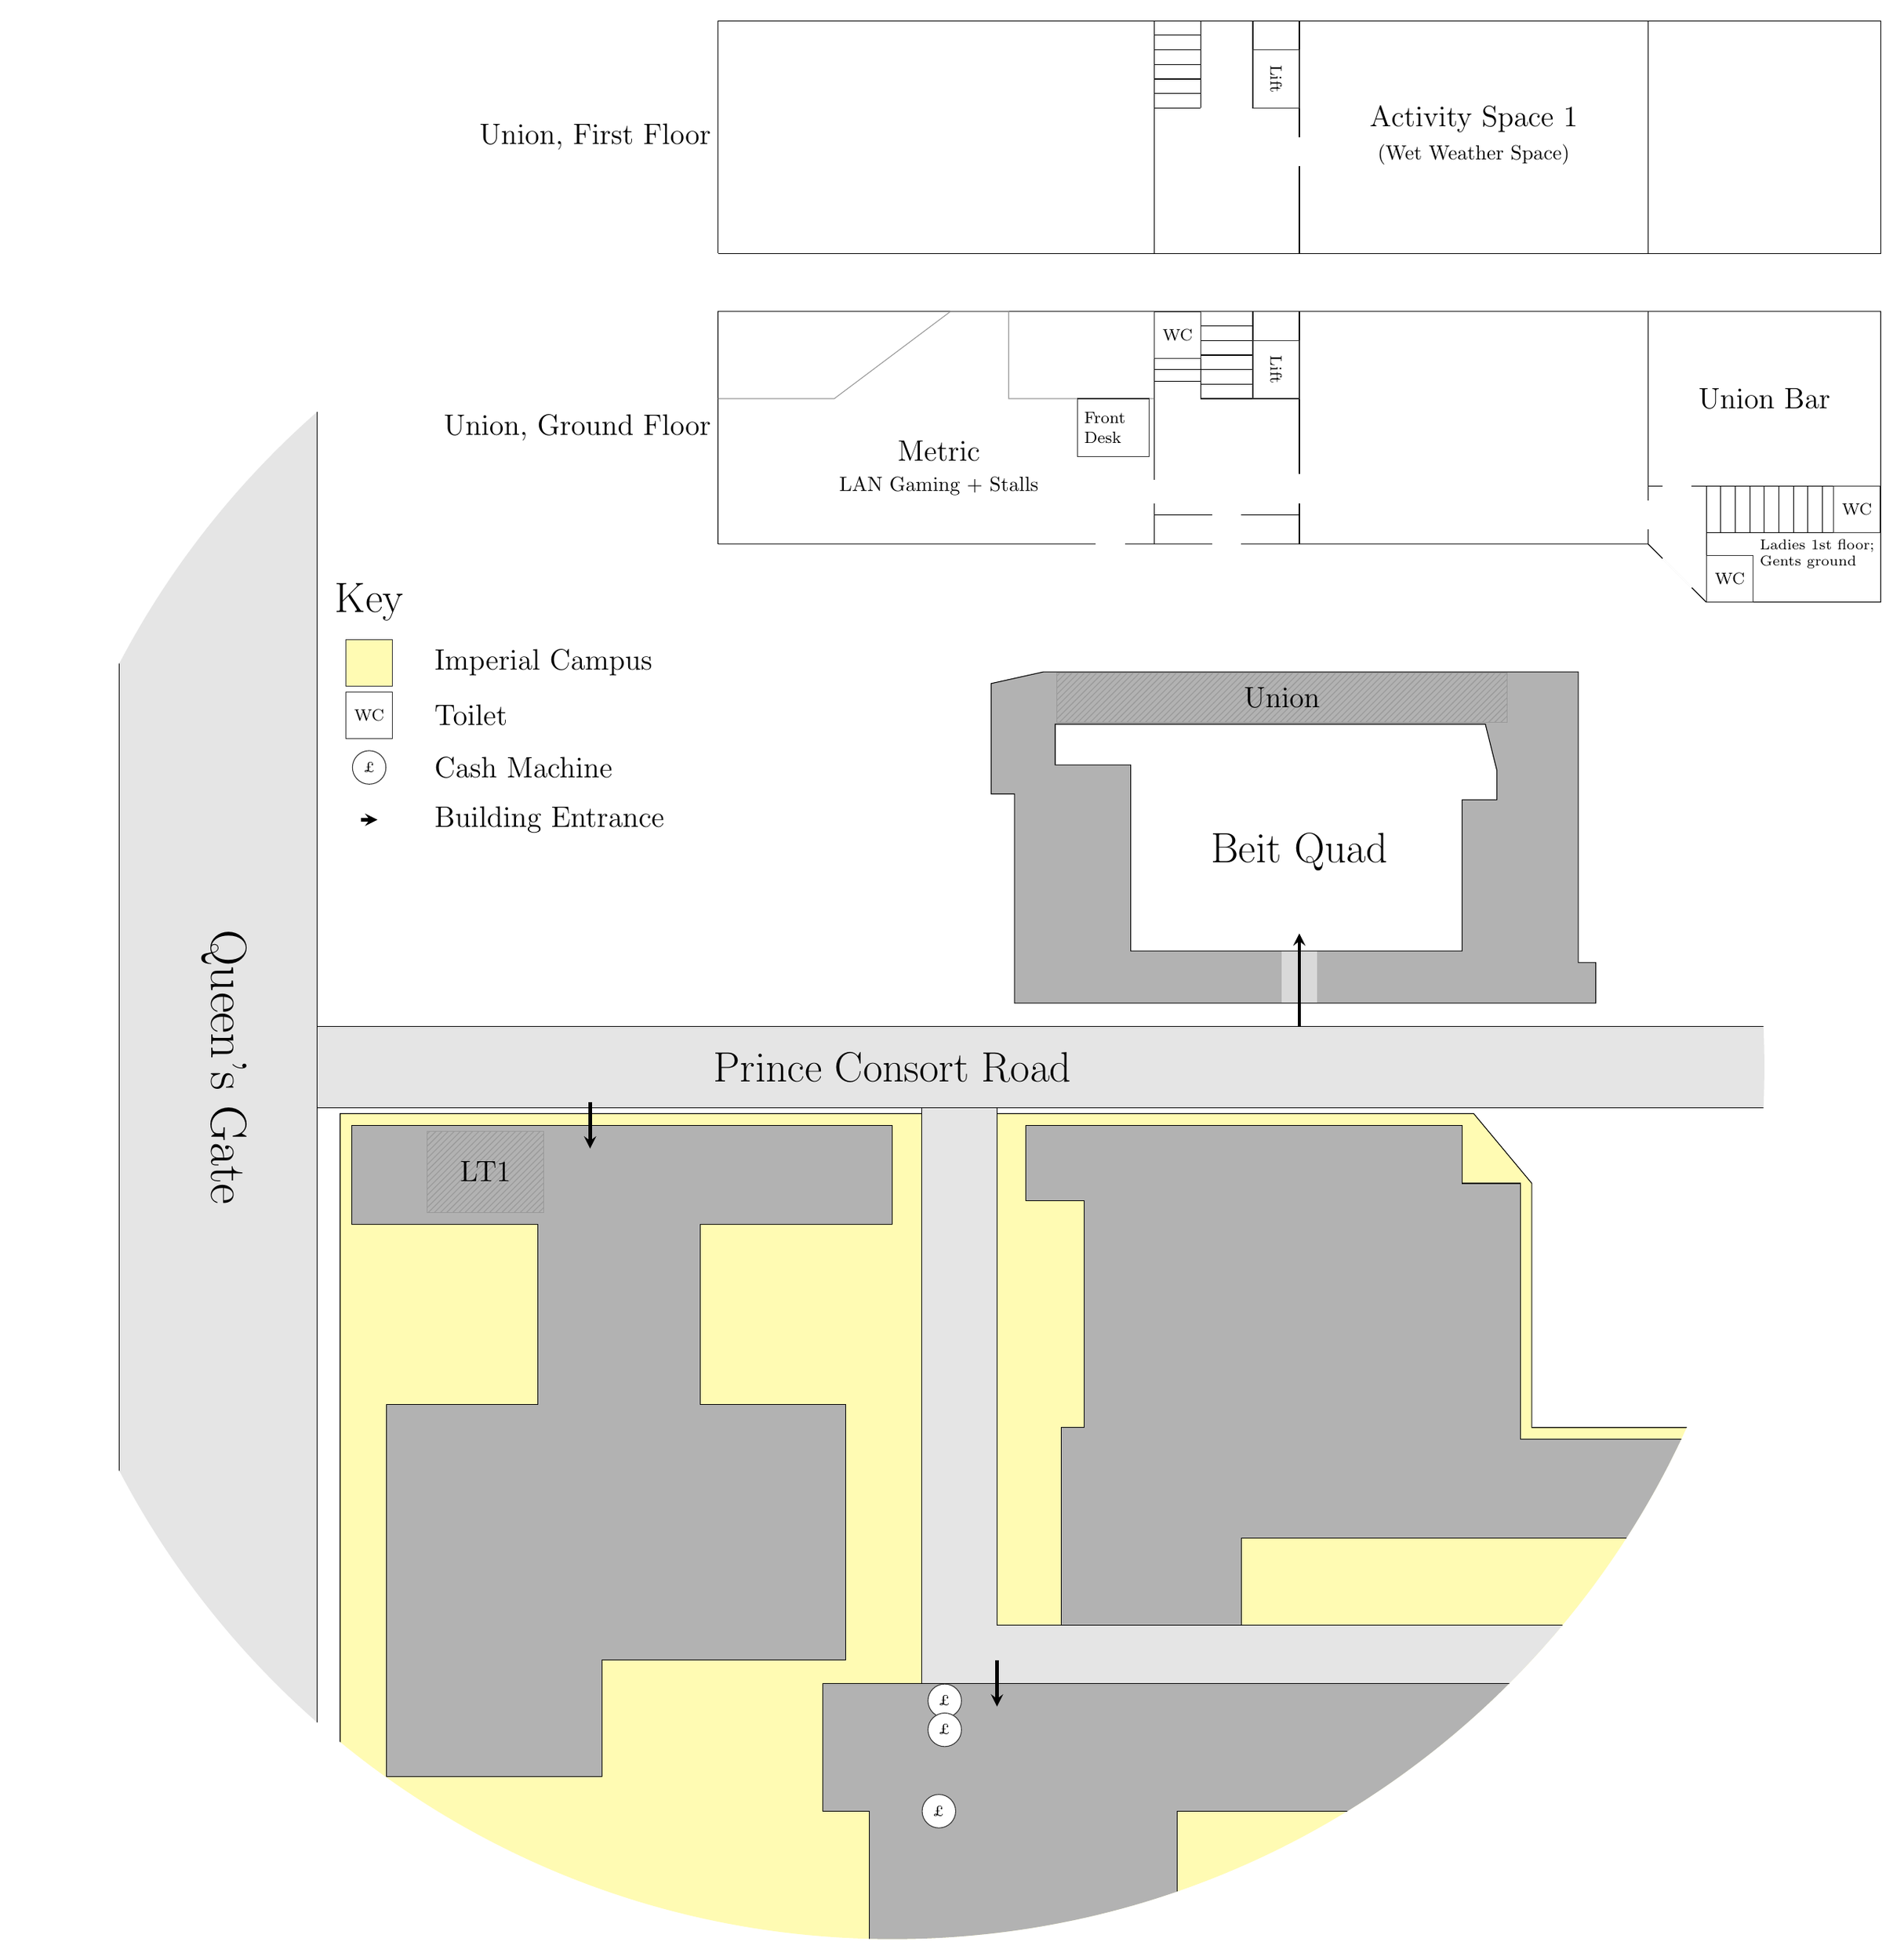
\begin{tikzpicture}

\begin{scope} % Campus Map {{{
\clip (-7,-2) circle (15);

%  Key {{{
\node (key) at (-16, 6) [font=\huge] {Key};
\begin{scope}[font=\Large,minimum height=\baselineskip,minimum width=\baselineskip];

	\node at ([below=6mm] key.south) [minimum width=8mm,minimum height=8mm,fill=yellow!30,draw=black!80] {};
	\node at ([below=6mm, right=10mm] key.south) [right] {Imperial Campus};

	\node at ([below=15mm] key.south) [minimum width=8mm,minimum height=8mm,fill=white,draw=black!80,font=\footnotesize] {WC};
	\node at ([below=15mm, right=10mm] key.south) [right] {Toilet};

	\node at ([below=24mm] key.south) [circle,fill=white,draw=black!80,font=\scriptsize] {\textsterling};
	\node at ([below=24mm, right=10mm] key.south) [right] {Cash Machine};

	\coordinate (entkey) at ([below=33mm] key.south);
	\draw [->,>=stealth,ultra thick] ([left=4pt] entkey) -- ([right=4pt] entkey);
	\node at ([below=33mm, right=10mm] key.south) [right] {Building Entrance};
\end{scope}
%}}}

% Beit Quad (Outer) {{{
\draw[fill=gray!60]
		(  5.1, - 0.9) --
		(  5.1, - 0.2) --
		(  4.8, - 0.2) --
		(  4.8,   4.8) --
		(- 4.4,   4.8) --
		(- 5.3,   4.6) --
		(- 5.3,   2.7) --
		(- 4.9,   2.7) --
		(- 4.9, - 0.9) --
		cycle
	; %}}}

% Beit Quad (Archway) {{{
\draw[fill=gray!30,draw=gray!30]
		(- 0.3, - 0.88) --
		(- 0.3,   0.01) --
		(  0.3,   0.01) --
		(  0.3, - 0.88) --
		cycle
	; %}}}

% Beit Quad (Inner) {{{
\draw[fill=white]
		(  2.8,   2.6) --
		(  3.4,   2.6) --
		(  3.4,   3.1) --
		(  3.2,   3.9) --
		(- 4.2,   3.9) --
		(- 4.2,   3.2) --
		(- 2.9,   3.2) --
		(- 2.9,   0.0) --
		(  2.8,   0.0) --
		cycle
	; %}}}

\node at ( 0,  1.7) [font=\huge] {Beit Quad};

\node[minimum width=7.75cm,minimum height=0.85cm,font=\Large,
	pattern=north east lines,pattern color=black!40,draw=black!40]
	at (-0.3,4.36) {Union};

%  Imperial Campus {{{
\draw[fill=yellow!30]
		(-16.5, - 2.8) --
		(  3.0, - 2.8) --
		(  4.0, - 4.0) --
		(  4.0, - 8.2) --
		( 10.0, - 8.2) --
		( 10.0, - 2.8) --
		( 20.0, - 2.8) --
		( 20.0, -21.0) --
		(-16.5, -21.0) --
		cycle
	; %}}}

% Blackett / Huley {{{
\draw[fill=gray!60]
		(-16.3, - 3.0) --
		(-16.3, - 4.7) --
		(-13.1, - 4.7) --
		(-13.1, - 7.8) --
		(-15.7, - 7.8) --
		(-15.7, -14.2) --
		(-12.0, -14.2) --
		(-12.0, -12.2) --
		(- 7.8, -12.2) --
		(- 7.8, - 7.8) --
		(-10.3, - 7.8) --
		(-10.3, - 4.7) --
		(- 7.0, - 4.7) --
		(- 7.0, - 3.0) --
		cycle
	; %}}}

\node [minimum height=1.4cm,minimum width=2cm,pattern=north east lines,
	pattern color=black!40,draw=black!40,font=\Large]
	at (-14, -3.8) {LT1};

% That Random Building (Group) {{{
\draw[fill=gray!60]
		(- 4.7, - 4.3) --
		(- 3.7, - 4.3) --
		(- 3.7, - 8.2) --
		(- 4.1, - 8.2) --
		(- 4.1, -11.6) --
		(- 1.0, -11.6) --
		(- 1.0, -10.1) --
		( 10.0, -10.1) --
		( 10.0, - 8.4) --
		(  3.8, - 8.4) --
		(  3.8, - 4.0) --
		(  2.8, - 4.0) --
		(  2.8, - 3.0) --
		(- 4.7, - 3.0) --
		cycle
	; %}}}

% Sherfield / Library {{{
\draw[fill=gray!60]
		( 13.4, -12.6) --
		(- 8.2, -12.6) --
		(- 8.2, -14.8) --
		(- 7.4, -14.8) --
		(- 7.4, -17.2) --
		(- 8.0, -17.2) --
		(- 8.0, -20.3) --
		(- 1.1, -20.3) --
		(- 1.1, -17.2) --
		(- 2.1, -17.2) --
		(- 2.1, -14.8) --
		( 13.4, -14.8) --
		cycle
	; %}}}

% Calendar Road {{{
\draw[fill=gray!20]
		(- 6.5, -12.6) --
		(  5.2, -12.6) --
		(  5.2, -11.6) --
		(- 5.2, -11.6) --
		(- 5.2, - 2.7) --
		(- 6.5, - 2.7) --
		cycle
	; %}}}

% Prince Consort Road {{{
\draw[fill=gray!20]
		( 23.3, - 1.3) --
		(-17.5, - 1.3) --
		(-17.5, - 2.7) --
		( 23.3, - 2.7) --
		cycle
	; %}}}

\node at (-7, -2) [font=\huge] {Prince Consort Road};

% Queen's Gate {{{
\draw[fill=gray!20]
		(-16.9, -18.7) --
		(-16.9, 15.3) --
		(-20.3, 15.3) --
		(-20.3, -18.7) --
		cycle
	; %}}}

\node at (-18.5, -2) [rotate=-90,font=\Huge] {Queen's Gate};

% Useful Entrances
\draw[->,>=stealth,ultra thick] (0, - 1.3) -- (0,  0.3); % Beit
\draw[<-,>=stealth,ultra thick] (-5.2,-13.0) -- (-5.2,-12.2); % Sherfield
\draw[<-,>=stealth,ultra thick] (-12.2,-3.4) -- (-12.2,-2.6); % Blackett

\end{scope} %}}}

\begin{scope}[shift={(-10,7)}] % Union Floor G Map {{{

	\draw (0, 0) -- (16, 0) -- (17, -1) -- (20, -1) -- (20, 4) -- (0, 4) -- (0,0) node [pos=0.5,left,font=\Large] {Union, Ground Floor};

	\draw (7.5, 0.5) -- (10, 0.5); % Inner Doors
	\draw (7.5,  0) -- (7.5,  4); % Metric / Hall
	\draw (10, 0) -- (10, 4); % Hall / 568
	\draw (16, 0) -- (16, 4); % 568 / Union Bar
	\draw (16, 1) -- (20, 1); % South of Union Bar
	\draw (17,-1) -- (17, 1); % East of NE corner entrance

	% NE steps to ladies
	\foreach \x in {17.25,17.5,17.75,18,18.25,18.5,18.75,19}{
		\draw (\x, 1) -- (\x, 0.2);
	}
	\draw (17, 0.2) -- (19.25, 0.2);

	% Main staircase
	\foreach \y in {2.5, 2.75, 3, 3.25, 3.5, 3.75}{
		\draw (8.3,\y) -- (9.2,\y);
	}
	\draw (8.3, 2.5) -- (8.3, 4);
	\draw (9.2, 2.5) -- (9.2, 4);

	% Stairs down to 'ground floor' toilets
	\foreach \y in {2.8, 3, 3.2}{
		\draw (7.5,\y) -- (8.3,\y);
	}

	% Main lift
	\node at (9.6, 3) [rotate=-90,font=\footnotesize,minimum height=8mm,minimum width=10mm,draw=black!80] {Lift};

	% Toilets
	\node at (7.5,4) % Main entry, both (steps! :/)
		[below right,minimum width=8mm,minimum height=8mm,fill=white,draw=black!80,font=\footnotesize] {WC};
	\node at (20,1) % NE, Ladies (1st Floor)
		[below left,minimum width=8mm,minimum height=8mm,fill=white,draw=black!80,font=\footnotesize] {WC};
	\node at (17,-1) % NE, Gents (outside Union Bar)
		[above right,minimum width=8mm,minimum height=8mm,fill=white,draw=black!80,font=\footnotesize] {WC};
	\node at (17.8,0.2) [below right,text width=2cm,font=\scriptsize] {Ladies 1st floor;\\ Gents ground};

	% Doors
	\begin{scope}[draw=white!100,thick]
		\draw (8.5,0) -- (9,0); % Main entrance
		\draw (8.5,0.5) -- (9,0.5); % Main entrance inner

		\draw (6.5,0) -- (7,0); % Metric external
		\draw (7.5,0.7) -- (7.5,1.1); % Metric internal

		\draw (10,0.7) -- (10,1.2); % 568 Internal

		\draw (16,0.25) -- (16,0.75); %568 <-> NE
		\draw (16.25,-0.25) -- (16.75,-0.75); % NE External
		\draw (16.25,1) -- (16.75,1); % Union bar
	\end{scope}

	% Rooms
	\node at (18,2.5) [font=\Large] {Union Bar};
	\node (met) at (3.8,1.6) [font=\Large] {Metric};
	\node at ([below=0.6cm] met) {LAN Gaming + Stalls};

	% Metric detailing
	\draw [draw=black!40] (7.5,2.5) -- (5,2.5) -- (5, 4) -- (4,4) -- (2,2.5) -- (0,2.5);
	\node at (6.8,2) [draw=black!80,text width=1cm,minimum width=1cm,minimum height=1cm,font=\footnotesize] {Front Desk};
\end{scope} %}}}

\begin{scope}[shift={(-10,12)}] % Union Floor 1 Map {{{

	\draw (0, 0) -- (20, 0) -- (20, 4) -- (0, 4) -- (0,0) node [pos=0.5,left,font=\Large] {Union, First Floor};

	\draw (7.5,  0) -- (7.5,  4); % Metric / Hall
	\draw (10, 0) -- (10, 4); % Hall / 568
	\draw (16, 0) -- (16, 4); % 568 / Union Bar

	\foreach \y in {2.5, 2.75, 3, 3.25, 3.5, 3.75}{
		\draw (7.5,\y) -- (8.3,\y);
	}
	\draw (8.3, 2.5) -- (8.3, 4);
	\draw (9.2, 2.5) -- (9.2, 4);
	\node at (9.6, 3) [rotate=-90,font=\footnotesize,minimum height=8mm,minimum width=10mm,draw=black!80] {Lift};

	% Doors
	\begin{scope}[draw=white!100,thick]
		\draw (10, 1.5) -- (10, 2);
	\end{scope}

	\node (as1) at (13, 2.3) [font=\Large] {Activity Space 1};
	\node at ([below=0.6cm] as1) {(Wet Weather Space)};
\end{scope} %}}}

% Cash Points {{{
\node at (- 6.1,-12.9) [circle,fill=white,draw=black!80,font=\scriptsize] {\textsterling};
\node at (- 6.1,-13.4) [circle,fill=white,draw=black!80,font=\scriptsize] {\textsterling};
\node at (- 6.2,-14.8) [circle,fill=white,draw=black!80,font=\scriptsize] {\textsterling};
%}}}

\end{tikzpicture}

}
	\end{center}
\end{article}

\end{document}
